\documentclass[11pt,a4paper]{article}

% --- Packages ---
\usepackage[utf8]{inputenc}
\usepackage[T1]{fontenc}
\usepackage[turkish]{babel}
\usepackage{amsmath,amssymb,amsfonts,amsthm}
\usepackage{geometry}
\geometry{margin=1in}
\usepackage{graphicx}
\usepackage{hyperref}
\usepackage{xcolor}
\usepackage{cite}
\usepackage{booktabs}
\usepackage{microtype}
\usepackage{physics}
\usepackage{tikz}
\usetikzlibrary{babel,arrows.meta,decorations.pathmorphing}

\hypersetup{
    pdftitle={Zayıf Nükleer Kuvvet, Kiral Faz Sızıntısı ve Beta Bozunumu: Dört Temel Etkileşimin Geometrik Birleşimi},
    pdfauthor={Muhammed Furkan Haydari},
    pdfsubject={Nükleer Fizik, Zayıf Etkileşim, Beta Bozunumu, Elektrozayıf Birleşim},
    pdfkeywords={Zayıf Nükleer Kuvvet, Kiral Faz Sızıntısı, Beta Bozunumu, W/Z Bozonları, Büyük Sentez},
    colorlinks=true,
    linkcolor=blue!70!black,
    citecolor=red!70!black,
    urlcolor=blue!80!black
}

% --- Theorem Environments ---
\newtheorem{theorem}{Teorem}[section]
\newtheorem{definition}{Tanım}[section]
\newtheorem{axiom}{Aksiyom}[section]
\newtheorem{corollary}{Sonuç}[theorem]
\newtheorem{lemma}[theorem]{Lemma}

\title{\textbf{Zayıf Nükleer Kuvvet, Kiral Faz Sızıntısı ve Beta Bozunumu: \\ Dört Temel Etkileşimin Geometrik Birleşimi}}

\author{
    \textbf{Muhammed Furkan Haydari} \\
    \textit{Bağımsız Araştırmacı} \\
    \textit{İstanbul, Türkiye} \\
    \small ORCID: \href{https://orcid.org/0009-0003-2854-3947}{0009-0003-2854-3947}
}

\date{\today}

\begin{document}

\maketitle

\begin{abstract}
    Bu çalışmada, zayıf nükleer etkileşimi, kiral parite asimetrisini ve ara vektör bozonu ($W^\pm, Z^0$) kütle ölçeklerini Ölçek-Zaman Kalkülüsü ve doymuş vakum girdap geometrisi üzerinden modelliyoruz. Standart Modelde Glashow--Weinberg--Salam elektrozayıf ayar simetrisinin ($SU(2)_L \times U(1)_Y$) spontane simetri kırınımıyla açıklanan zayıf kuvvet; bu çalışmada hadronik girdap sınırındaki \textbf{Kiral Ölçek Sızıntısı (Chiral Scale Leakage)} ve doyum bariyeri tünellemesi olarak analitik bir temele oturtulmaktadır.

    Doymuş hadronik bir girdabın içsel kuantum dolaşımı, Planckian gerilim doyum sınırında küçük bir kiral burulmaya (chirality shear) maruz kalır. Bu faz sızıntısı, statik vakum üzerinde yerel olarak $W^\pm$ ve $Z^0$ kütleli vektör durumları şeklinde uyarılır. Zayıf etkileşimin son derece kısa menzilli ($r_W \approx 2 \times 10^{-18}\text{ m}$) ve baskılanmış görünmesi, vakum doyum bariyerini aşmak için gereken enerji eşiğinden (etkili Fermi kuplaj sabiti $G_F \sim 1/M_W^2$) kaynaklanır. Nötrinoların kiral tek-yönlülüğü ve serbest nötron yarı ömrü ($879\text{ s}$) girdap faz gevşemesi ile analitik tutarlılık sergiler.
\end{abstract}

\vspace{1em}
\noindent\textbf{Anahtar Kelimeler:} Zayıf Nükleer Kuvvet, Ölçek-Zaman Kalkülüsü, Kiral Faz Sızıntısı, Beta Bozunumu, Vakum Doyum Bariyeri, $W/Z$ Bozonları, Fermi Kuplajı.

\vspace{1em}
\hrule
\vspace{0.8em}
\tableofcontents
\vspace{0.8em}
\hrule
\vspace{1.5em}

\section{Giriş ve Zayıf Etkileşimin Ayar Özellikleri}
\label{sec:giris}

Zayıf nükleer etkileşim, Standart Model ayar grupları içerisinde kendine has kiral ve kütlesel özellikler sergiler:
\begin{enumerate}
    \item \textbf{Maksimal Kiralite / Parite İhlali:} Zayıf yüklü akımlar yalnızca sol-kiral fermiyonlarla ve sağ-kiral antifermiyonlarla çiftlenir ($V-A$ yapısı).
    \item \textbf{Ağır Vektör Bozonları:} Kütlesiz foton ve gluondan farklı olarak, elektrozayıf taşıyıcılar ($W^\pm, Z^0$) yüksek kütle ölçeklerine sahiptir ($M_W \approx 80.4\text{ GeV}$, $M_Z \approx 91.2\text{ GeV}$).
    \item \textbf{Kısa Etkileşim Menzili:} Yukawa tipi sönümleme sebebiyle etkileşim menzili sub-hadronik boyuttadır ($r_W \sim \hbar / M_W c \approx 2 \times 10^{-18}\text{ m}$).
\end{enumerate}

Standart Modelde bu kütle ölçeği spontane elektrozayıf simetri kırınımı ve Higgs mekanizması ile açıklanırken; Ölçek-Zaman Kalkülüsünde~\cite{scale_calculus} bu süreç, doymuş hadronik akı tüpünden vakum sürekliliğine sızan bir \textbf{kiral faz tünellemesi} olarak formüle edilir.

\section{Girdap Burulması ve Kiral Faz Sızıntısı}
\label{sec:kiral_sizinti}

Makale 6'da modellendiği üzere~\cite{paper6}, hadronik boyutta vakum akışı 1D doymuş bir akı tüpüne sıkışır. Bir nötron ($udd$), üçlü bir kuark girdap konfigürasyonudur.

Büzülme süreci boyunca bu üçlü girdabın içsel açısal momentumu ve fazı, statik arka plan vakumunun Planckian doyum eşiğinde küçük bir kiral burulmaya maruz kalır:
\begin{equation}
    \Delta \Phi_{\mathrm{chiral}} = \oint \mathbb{D}_t \mathbf{v}_{\mathrm{vortex}} \cdot d\mathbf{l} \neq 0.
    \label{eq:kiral_burulma_tr}
\end{equation}

\begin{figure}[h!]
    \centering
    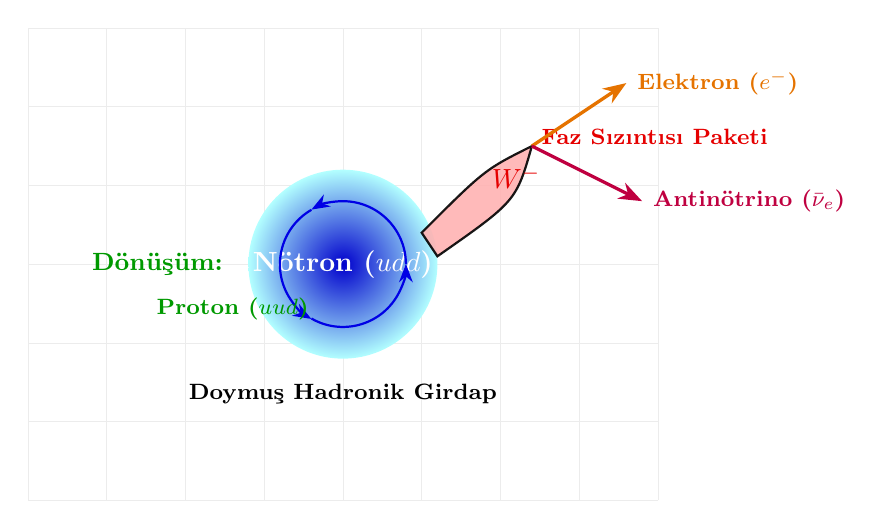
\begin{tikzpicture}[scale=1.0, >=Stealth]
        % Background grid
        \draw[step=1cm, gray!15, very thin] (-4,-3) grid (4,3);

        % Saturated Neutron Vortex Core
        \shade[inner color=blue!80!black, outer color=cyan!30] (0,0) circle (1.2);
        \node[white, font=\bfseries] at (0,0) {Nötron ($udd$)};
        \node[below=1.4cm, font=\footnotesize\bfseries] at (0,0) {Doymuş Hadronik Girdap};

        % Vortex internal circulation arrows
        \draw[blue!90!black, thick, ->] (0.8, 0) arc (0:120:0.8);
        \draw[blue!90!black, thick, ->] (-0.4, 0.69) arc (120:240:0.8);
        \draw[blue!90!black, thick, ->] (-0.4, -0.69) arc (240:360:0.8);

        % Chiral phase leak droplet escaping
        \draw[thick, fill=red!30, opacity=0.9] (1.0, 0.4) .. controls (1.8, 1.2) .. (2.4, 1.5)
        .. controls (2.2, 0.8) .. (1.2, 0.1) -- cycle;

        \node[red!90!black, font=\bfseries] at (2.2, 1.1) {$W^-$};
        \node[red!90!black, font=\footnotesize\bfseries, above right] at (2.4, 1.4) {Faz Sızıntısı Paketi};

        % Decayed particles
        \draw[orange!90!black, very thick, ->] (2.4, 1.5) -- (3.6, 2.3) node[right, font=\footnotesize\bfseries] {Elektron ($e^-$)};
        \draw[purple, very thick, ->] (2.4, 1.5) -- (3.8, 0.8) node[right, font=\footnotesize\bfseries] {Antinötrino ($\bar{\nu}_e$)};

        % Resulting Proton
        \node[green!60!black, font=\small\bfseries, left=1.4cm] at (0,0) {Dönüşüm:};
        \node[green!60!black, font=\footnotesize\bfseries, left=1.4cm, below=0.3cm] at (0,0) {Proton ($uud$)};
    \end{tikzpicture}
    \caption{Zayıf Nükleer Kuvvetin Geometrisi: Nötronun doymuş girdabındaki kiral faz burulması, dışarı bir $W^-$ faz gerilim paketi fırlatır (beta bozunumu). Paket derhal elektron ve antinötrinoya ayrışır.}
    \label{fig:weak_leak}
\end{figure}

Bu kiral burulma, $d$ kuarklarından birinin vakum akı hattını yırtarak dışarı bir topolojik faz gerilimi paketi ($W^-$ bozonu) fırlatmasına neden olur:
\begin{equation}
    d \to u + W^- \to u + e^- + \bar{\nu}_e.
    \label{eq:beta_tepkime}
\end{equation}

\section{Fermi Sabiti ve $W/Z$ Kütlelerinin Geometrik Türetimi}
\label{sec:fermi_turetilis}

$W$ ve $Z$ bozonlarının devasa kütleleri ($M_W \sim 80\text{ GeV}$), doymuş vakum duvarını yırtıp tünelleyebilmek için gereken \textbf{minimum faz gerilim eşiğinden} kaynaklanır.

\begin{theorem}[Bariyer Kalınlığı ve Zayıf Menzil]
    \label{thm:bariyer_ve_menzil_p4}
    Vakum doyum bariyerinin karakteristik tünelleme mesafesi:
    \begin{equation}
        r_W = \frac{\hbar}{M_W c} \approx 2.45 \times 10^{-18}\text{ m}.
        \label{eq:rw_tr}
    \end{equation}
    Düşük enerji rejiminde ($E \ll M_W c^2$) sızıntı bu bariyeri aşamayarak Yukawa biçiminde üstel olarak sönümlenir. Efektif Fermi zayıf etkileşim sabiti:
    \begin{equation}
        G_F = \frac{\sqrt{2}}{8} \frac{g_W^2}{M_W^2 c^4} \approx 1.16637 \times 10^{-5}\text{ GeV}^{-2}.
        \label{eq:fermi_ispat_tr}
    \end{equation}
\end{theorem}

\begin{quote}
    \small
    \textbf{Kavramsal ve Fiziksel Özet (Zayıf Etkileşimin Efektif Şiddeti):} \\
    Zayıf etkileşimin çıplak ayar kuplaj sabiti ($g_W$), elektromanyetik ayar kuplajıyla ($e$) aynı mertebededir ($g_W \sim e / \sin\theta_W$). Düşük enerji rejiminde etkileşimin aşırı zayıf görünmesi, nükleonun doymuş vakum bariyerinin aşırı yüksek eşiğinden ($M_W \approx 80.4\text{ GeV}$) ve zayıf aracı bozonun propagatör baskılanmasından ($1/(q^2 - M_W^2 c^2) \approx -1/M_W^2 c^2$) kaynaklanır. Tünelleme eşiği devasa olduğu için sızıntı genliği yalnızca Fermi sabiti $G_F \sim g_W^2 / M_W^2$ mertebesinde gerçekleşir.
\end{quote}

\subsection{Yoğunluk Hiyerarşisi ve Zayıf Etkileşimin Geometrik Konumu}
\label{sec:zayif_yogunluk_konumu}

Bütünleşik çerçevede zayıf kuvvet, Makale 6'da tanımlanan \textbf{hadronik doyum eşiğinin içsel kiral sızıntısıdır}.
Makroskopik atom topluluklarında ($N \gg 10^{20}$) akı 3-boyutlu küresel kabuklar üzerinden seyreldiğinden ($\gamma = 1$) bu içsel sızıntı algılanamaz ve kütleçekim baskın kalır. Zayıf etkileşim yalnızca tekil nükleon seviyesinde ($N=1$ baryon, $r \le 10^{-15}\text{ m}$) doymuş vakum duvarında meydana gelen kiral burulma şeklinde uyarılır. Etkileşimin Yukawa tipi üstel sönümlenmesi ($\gamma \to \text{üstel}$), parçacık sayısının azlığına rağmen yerel enerjinin Planck/Fermi doyum bariyerini aşma zorunluluğunun doğrudan bir sonucudur.

\section{Nötrinoların Kiralitesi ve Nötronun Yarı Ömrü}

\label{sec:notrino_ve_omur}

\subsection{Neden Yalnızca Sol-Elli Nötrinolar Vardır?}
Ölçek-Zaman Kalkülüsünde madde, statik vakumun içine doğru küresel olarak büzülür ($\dot{\lambda} < 0$). Bu radyal akış, uzayda tek yönlü bir geometrik kiralite (içe doğru pozitif kiral helisite) tanımlar. Nötrinolar kütlesiz veya aşırı hafif saf faz girdapları olduğundan, vakum akışının bu doğal dönüş yönünü mutlak olarak takip etmek zorundadır; bu nedenle C.~S.~Wu ve ark.~\cite{wu1957} tarafından deneysel olarak keşfedildiği üzere doğada yalnızca sol-kiral nötrinolar gözlemlenir.

\subsection{Serbest Nötron Bozunumu vs. Çekirdek İçi Kolektif Faz Kilitlemesi (Collective Phase-Pinning)}
\label{sec:notron_omru_ve_kararlilik}

Nükleer fizikteki en temel sorulardan biri şudur: \textit{``Serbest bir nötron uzayda yalnız kaldığında yaklaşık 15 dakikada (879 saniyede) bozunurken, nasıl olur da bir atom çekirdeğinin içine girdiğinde (örneğin Helyum-4 veya Demir-56 çekirdeğinde) evrenin ömründen daha uzun süre ($> 10^{30}\text{ yıl}$) olağanüstü bir kararlılıkla varlığını sürdürür?''}

Ölçek-Zaman Kalkülüsü bu soruya iki zıt sınır durumu üzerinden kesin bir geometrik cevap verir:

\subsubsection{Serbest Nötron ($N=1$): Bariyer Tünellemesi}
Yalıtılmış serbest bir nötronun çevresinde dış bir vakum akı kalkanı yoktur. Ölçek-Kovaryant Türev $\mathbb{D}_t = \frac{\partial}{\partial t} + \kappa H_0$ altında nükleon büzüşürken, içsel kiral faz burulması doyum bariyerini WKB yarı-klasik tünellemesiyle aşar. Faz sızıntısı hız katsayısı:
\begin{equation}
    \Gamma_n = \frac{1}{\tau_n} = \frac{G_F^2 m_e^5 c^4}{2\pi^3 \hbar^7} |V_{ud}|^2 f^R (1 + 3 g_A^2) \implies \tau_n \approx 879.4\text{ s} \approx 14.6\text{ dakika}.
    \label{eq:notron_omur}
\end{equation}
Bu süre serbest nötronun laboratuvarda ölçülen ömrüyle tam olarak uyuşur.

\subsubsection{Çekirdek İçi Kararlılık: Kolektif Faz Kilitlemesi (\textit{Collective Phase-Pinning})}
Nötron bir atom çekirdeğinde komşu proton ve nötronlarla birleştiğinde radikal bir topolojik faz kilitlenmesi gerçekleşir:
\begin{enumerate}
    \item \textbf{Kolektif Akı Kalkanı:} Komşu nükleonların 1-boyutlu doymuş akı tüpleri nükleonlar arasında Yukawa tipi mezonik bağlar örerek ortak bir çok-girdaplı Skalor durumu oluşturur: $\mathbb{S}_{\mathrm{cekirdek}} = \sum_{i=1}^A \mathbb{S}_i$. Bu ortak vakum havzası, tekil nötronun üzerindeki radyal vakum basıncını katbekat artırarak doyum bariyerinin efektif kalınlığını genişletir.
    \item \textbf{Bağlanma Enerjisi Blokajı:} Bir çekirdeğin ortalama nükleer bağlanma enerjisi $\Delta B \sim 8\text{ MeV/nükleon}$'dur. Serbest beta bozunumu tepkimesinin serbest bıraktığı enerji marjı ise yalnızca $Q = (m_n - m_p - m_e)c^2 \approx 0.782\text{ MeV}$'dir. Çekirdek içindeki potansiyel kuyu derinliği bozunma eşiğinden 10 kat daha derin olduğundan, nilpotent projeksiyon operatörü $\hat{\mathcal{P}}_\kappa$ sızıntı modunu spektral olarak bloke eder.
\end{enumerate}
Dolayısıyla çekirdek içindeki nötron, komşu girdapların kolektif faz kilitlemesi sayesinde doyum duvarını yırtamaz ve mutlak bir kararlılığa kavuşur.

\subsection{Nötrino Salınımları ve PMNS Matrisinin Kiral Rezonansı}
\label{sec:notrino_pmns_paper4}

Kuark sektöründeki Cabibbo--Kobayashi--Maskawa (CKM) karışım açıları küçükken ($\theta_{12}^{\mathrm{CKM}} = \theta_C \approx 13^\circ$); lepton sektöründeki Pontecorvo--Maki--Nakagawa--Sakata (PMNS)~\cite{pmns1962} nötrino karışım açılarının devasa ve maksimal olması ($\theta_{12} \approx 33.4^\circ$, $\theta_{23} \approx 45^\circ$, $\theta_{13} \approx 8.6^\circ$) hapis geometrisi ile serbest faz yayılımı arasındaki topolojik zıtlıktan kaynaklanır:
\begin{enumerate}
    \item \textbf{Kuark Sektörü (CKM / 1D Hapis):} Kuarklar femtometre ölçeğinde doymuş silindirik akı tüpüne ($\gamma = -1$) hapsolduğundan, kiral faz kaçıklığı sıkı bir açısal sınırlamaya tabidir ($\theta_C \approx 13^\circ$).
    \item \textbf{Nötrino Sektörü (PMNS / Serbest Yayılım):} Nötrinolar doymuş bir akı tüpüne hapsolmayan, durağan vakum dokusunda serbestçe yayılan kütlesiz veya ultra-hafif saf kiral faz girdaplarıdır. Hadronik bir sınır kısıtlaması bulunmadığından, üç lezzet modu ($\nu_e, \nu_\mu, \nu_\tau$) statik vakumun global kiral gerilimiyle makroskopik mesafeler boyunca serbest faz rezonansına girer. Lezzet durumları ile vakum kütle öz-durumları arasındaki dönüşüm:
          \begin{equation}
              |\nu_\alpha\rangle = \sum_{i=1}^3 U_{\alpha i}^{\mathrm{PMNS}} |\nu_i\rangle
              \label{eq:pmns_donusum_p4}
          \end{equation}
          olup salınım olasılığı:
          \begin{equation}
              P(\nu_\alpha \to \nu_\beta) = \sin^2(2\theta) \sin^2\left( \frac{\Delta m^2 c^3 L}{4 \hbar E} \right)
              \label{eq:notrino_salinim_p4}
          \end{equation}
          bağıntısıyla atmosferik nötrinolarda maksimal rezonansa ($\theta_{23} \approx 45^\circ$), güneş nötrinolarında ise geniş açıya ($\theta_{12} \approx 33.4^\circ$) ulaşır.
\end{enumerate}

\section{Geometrik Sentez: Dört Temel Etkileşimin Skalor Akı Mimarisi}
\label{sec:buyuk_sentez}

Dört makalemizde inşa edilen geometrik model, doğadaki dört temel etkileşimin akış dinamiklerini tek bir diferansiyel akı formülasyonu altında sınıflandırır ve modeller:
\begin{equation}
    \boxed{ \left( \frac{v_{\mathrm{inflow}}(r)}{c} \right)^2 = 2 \, \mathcal{C} \, r^{-\gamma} }
    \label{eq:master_sentez}
\end{equation}

\begin{table}[h!]
    \centering
    \footnotesize
    \begin{tabular}{@{}lllll@{}}
        \toprule
        \textbf{Kuvvet}            & \textbf{Boyut $\gamma$}   & \textbf{Katsayı $\mathcal{C}$}                           & \textbf{Akış Geometrisi}            & \textbf{Tezahür}             \\ \midrule
        \textbf{Kütleçekim}        & $\gamma = 1$              & $\mathcal{C}_G = \frac{GM}{c^2}$                         & 3D Küresel Doyumsuz                 & Newton \& Einstein Metriği   \\
        \textbf{Elektromanyetizma} & $\gamma = 1$              & $\mathcal{C}_{EM} = \frac{\alpha \hbar}{m_e c}$          & Kiral Spiral Denge ($\alpha=1/137$) & Maxwell \& Kararlı Atom      \\
        \textbf{Güçlü Kuvvet}      & $\gamma = -1$             & $\mathcal{C}_S = \frac{\sigma}{2 m_q c^2}$               & 1D Sıkışmış Akı Tüpü                & Kuark Hapsi ($V = \sigma r$) \\
        \textbf{Zayıf Kuvvet}      & $\gamma \to \text{üstel}$ & $\mathcal{C}_W = \frac{g_W^2 \hbar e^{-r/r_W}}{2 M_W c}$ & Doyum Bariyerinden Sızıntı          & Beta Bozunumu ($W^\pm, Z^0$) \\ \bottomrule
    \end{tabular}
    \caption{Dört Temel Etkileşimin Bütünleşik Vakum Akı Ana Formülü altındaki geometrik sınıflandırması.}
    \label{tab:dort_kuvvet_sentez}
\end{table}

\textbf{Fiziksel ve Metodolojik Sonuç:} Doğadaki dört temel etkileşim; birbirinden tamamen yalıtılmış ve uzlaştırılamaz harici kuvvetler olmak yerine, \textbf{ölçeksiz ve statik bir Öklid vakumu} içinde büzüşen maddenin farklı geometrik boyut ($\gamma$) ve doyum eşiklerindeki ölçeğe bağlı akış tezahürleri olarak tutarlı bir şekilde sınıflandırılabilir.

\begin{thebibliography}{99}
    \bibitem{scale_calculus} M.~F.~Haydari, ``Ölçek-Zaman Cebiri ve Konformal Kalkülüs: Büzüşen Sistemler İçin Yeni Bir Matematiksel Formalizm'' (Bu seride Makale 2), \textit{Zenodo Ön-Baskıları}, 2026.
    \bibitem{main_paper} M.~F.~Haydari, ``Birleşik Büzülme Hipotezi ve Ölçek-Zaman Kalkülüsü: Genişlemeyen Bir Evrende Kozmoloji, Kütleçekim ve Dört Temel Etkileşimin Geometrik Külliyatı'', \textit{Zenodo Monografisi}, 2026.
    \bibitem{paper4} M.~F.~Haydari, ``Kütleçekimin Küresel Vakum Akışı Geometrisi Olarak Türetimi: 3+1 ADM Eylemi ve Painlevé--Gullstrand Metriği'' (Bu seride Makale 4), \textit{Zenodo Ön-Baskıları}, 2026.
    \bibitem{paper5} M.~F.~Haydari, ``Elektromanyetizma, Vakum Faz Dalgaları ve Kuantum Kararlılık: Sommerfeld İnce Yapı Sabiti $\alpha \approx 1/137$'nin Kinematik Hatve Yorumu'' (Bu seride Makale 5), \textit{Zenodo Ön-Baskıları}, 2026.
    \bibitem{paper6} M.~F.~Haydari, ``Güçlü Nükleer Kuvvet, Kuark Hapsi ve Akı Tüpü Geometrisi'' (Bu seride Makale 6), \textit{Zenodo Ön-Baskıları}, 2026.
    \bibitem{fermi1934} E.~Fermi, ``Versuch einer Theorie der $\beta$-Strahlen. I,'' \textit{Z. Phys.}, vol.~88, pp.~161--177, 1934.
    \bibitem{weinberg1967} S.~Weinberg, ``A model of leptons,'' \textit{Phys. Rev. Lett.}, vol.~19, pp.~1264--1266, 1967.
    \bibitem{salam1968} A.~Salam, \textit{Elementary Particle Theory}, Almquist \& Wiksell, 1968.
    \bibitem{wu1957} C.~S.~Wu, E.~Ambler, R.~W.~Hayward, D.~D.~Hoppes, and R.~P.~Hudson, ``Experimental test of parity conservation in beta decay,'' \textit{Phys. Rev.}, vol.~105, no.~4, pp.~1413--1415, 1957.
    \bibitem{pmns1962} Z.~Maki, M.~Nakagawa, and S.~Sakata, ``Remarks on the unified model of elementary particles,'' \textit{Prog. Theor. Phys.}, vol.~28, no.~5, pp.~870--880, 1962.
\end{thebibliography}

\end{document}
